%% LyX 2.3.4.2 created this file.  For more info, see http://www.lyx.org/.
%% Do not edit unless you really know what you are doing.
\documentclass[american]{beamer}
\usepackage{lmodern}
\renewcommand{\sfdefault}{lmss}
\renewcommand{\ttdefault}{lmtt}
\usepackage[T1]{fontenc}
\usepackage[latin9]{inputenc}
\usepackage{calc}
\usepackage{amstext}
\usepackage{amssymb}
\usepackage{graphicx}

\makeatletter
%%%%%%%%%%%%%%%%%%%%%%%%%%%%%% Textclass specific LaTeX commands.
% this default might be overridden by plain title style
\newcommand\makebeamertitle{\frame{\maketitle}}%
% (ERT) argument for the TOC
\AtBeginDocument{%
  \let\origtableofcontents=\tableofcontents
  \def\tableofcontents{\@ifnextchar[{\origtableofcontents}{\gobbletableofcontents}}
  \def\gobbletableofcontents#1{\origtableofcontents}
}

%%%%%%%%%%%%%%%%%%%%%%%%%%%%%% User specified LaTeX commands.
\usetheme[compress]{Berlin}
%\usecolortheme{dove}
\hypersetup{pdfpagemode=None,linkcolor=white}
\usepackage{tikz}
\usepackage{handoutWithNotes}

\usetikzlibrary{shapes.multipart}
\usetikzlibrary{decorations.pathreplacing}
%\pgfpagesuselayout{1 on 1 with notes landscape}[letterpaper,border shrink=5mm] 
\setbeamertemplate{navigation symbols}{}%remove navigation symbols


\usepackage{import}
\usepackage{upgreek}
\usepackage{bbold}
\usepackage{alltt}
\usepackage{bbm}

\renewcommand{\partname}{Lecture}

\makeatother

\usepackage{babel}
\begin{document}
\title[Simulation and Scopes]{Simulation and Scopes}
\subtitle{Proposal}
\author[Pupalaikis]{P.~Pupalaikis\inst{}}
\institute[{{\vspace{-1em}

\includegraphics[scale=0.1]{../Common/TeledyneLeCroyLogo}}}]{\inst{}Teledyne LeCroy\\
}
\titlegraphic{\noindent 
\includegraphics[scale=0.5]{../Common/TeledyneLeCroyLogo}}
\date[07/05/2021]{07/05/2021}

\makebeamertitle

%\pgfdeclareimage[height=0.25cm]{institution-logo}{TeledyneLeCroyLogo.png}
%\logo{\pgfuseimage{institution-logo}}

\AtBeginSubsection[]{%
  \frame<beamer>{ 
    \frametitle{Outline}   
    \tableofcontents[currentsection,currentsubsection] 
  }
}

%\beamerdefaultoverlayspecification{<+->}

\part{Simulation and Oscilloscopes}

%\frame{\partpage}
\begin{frame}{Outline}

\tableofcontents{}
\end{frame}

\section{Goal of this Presentation}
\begin{frame}{Goal of this Presentation}
\begin{itemize}
\item To present, from this user's perspective, the case for integrating
simulation tools with the oscilloscope software
\item To provide some examples that promote and facilitate this need.
\item Present practical technical details regarding where things stand today.
\end{itemize}
\end{frame}
%

\section*{Presentation}
\begin{frame}{Simulation in the Design Environment}
\begin{columns}[c]

\column{0.4\textwidth}

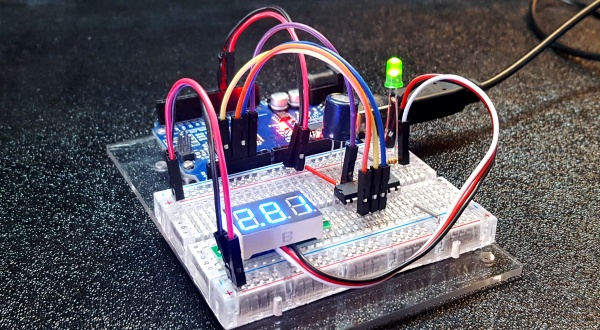
\includegraphics[width=1\columnwidth]{BreadBoard}

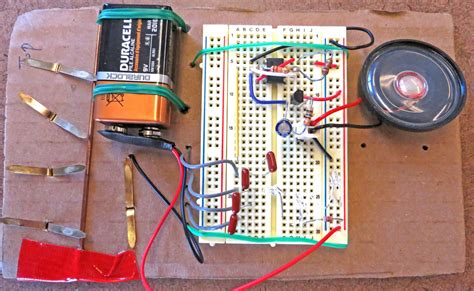
\includegraphics[width=1\columnwidth]{BreadBoard2}

\column{0.7\textwidth}
\begin{itemize}
\item It used to be common to breadboard circuits. In these cases, test
equipment would be employed to debug these prototypes
\item In today's world, the design of the prototype involves simulation.
Not only is the test equipment cut out of this development phase,
but the analysis software employed in high-end equipment, such as
high-speed oscilloscopes cannot be used
\end{itemize}
\end{columns}

\begin{block}{Oscilloscope software is trapped in the instrument and withheld from
simulation.}
\end{block}
\end{frame}
%
\begin{frame}{IC Design}
\begin{columns}

\column{0.4\textwidth}

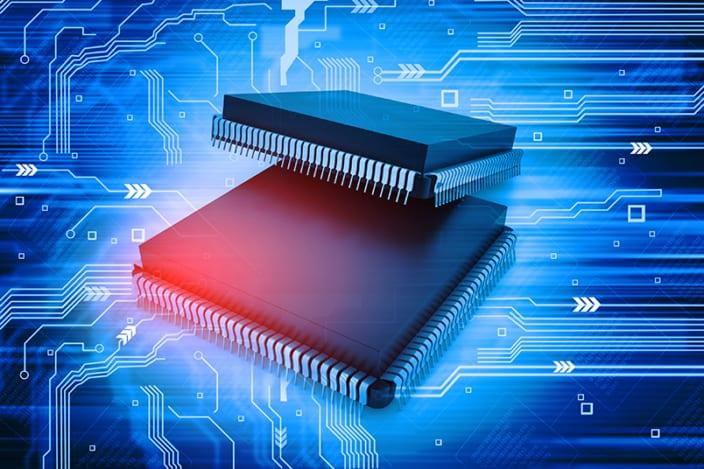
\includegraphics[width=1\columnwidth]{ICs}

\column{0.7\textwidth}
\begin{itemize}
\item IC design makes the situation worse \textendash{} they are only simulated.
\item The simulation is long, expensive, and the capability for analyzing
the results is particularly poor.
\end{itemize}
\end{columns}

\begin{block}{Furthermore, when evaluating design choices and trade-offs, a system
level view is desired, necessitating simulation of the constituent
elements of the system together to determine final system performance.
It is common to refine simulations more and more and the design progresses
to get an ever increasingly accurate view of the system.}
\end{block}
\end{frame}
%
\begin{frame}{A PDN Simulation}
\begin{columns}

\column{0.7\textwidth}

{\small{}A PDN model is created and simulated in HFSS to determine
the impedance vs. frequency, the model is fitted (to identify design
points of control, such as wire bond inductance), and a transient
simulation shows the supply noise.}{\small\par}

\begin{figure}
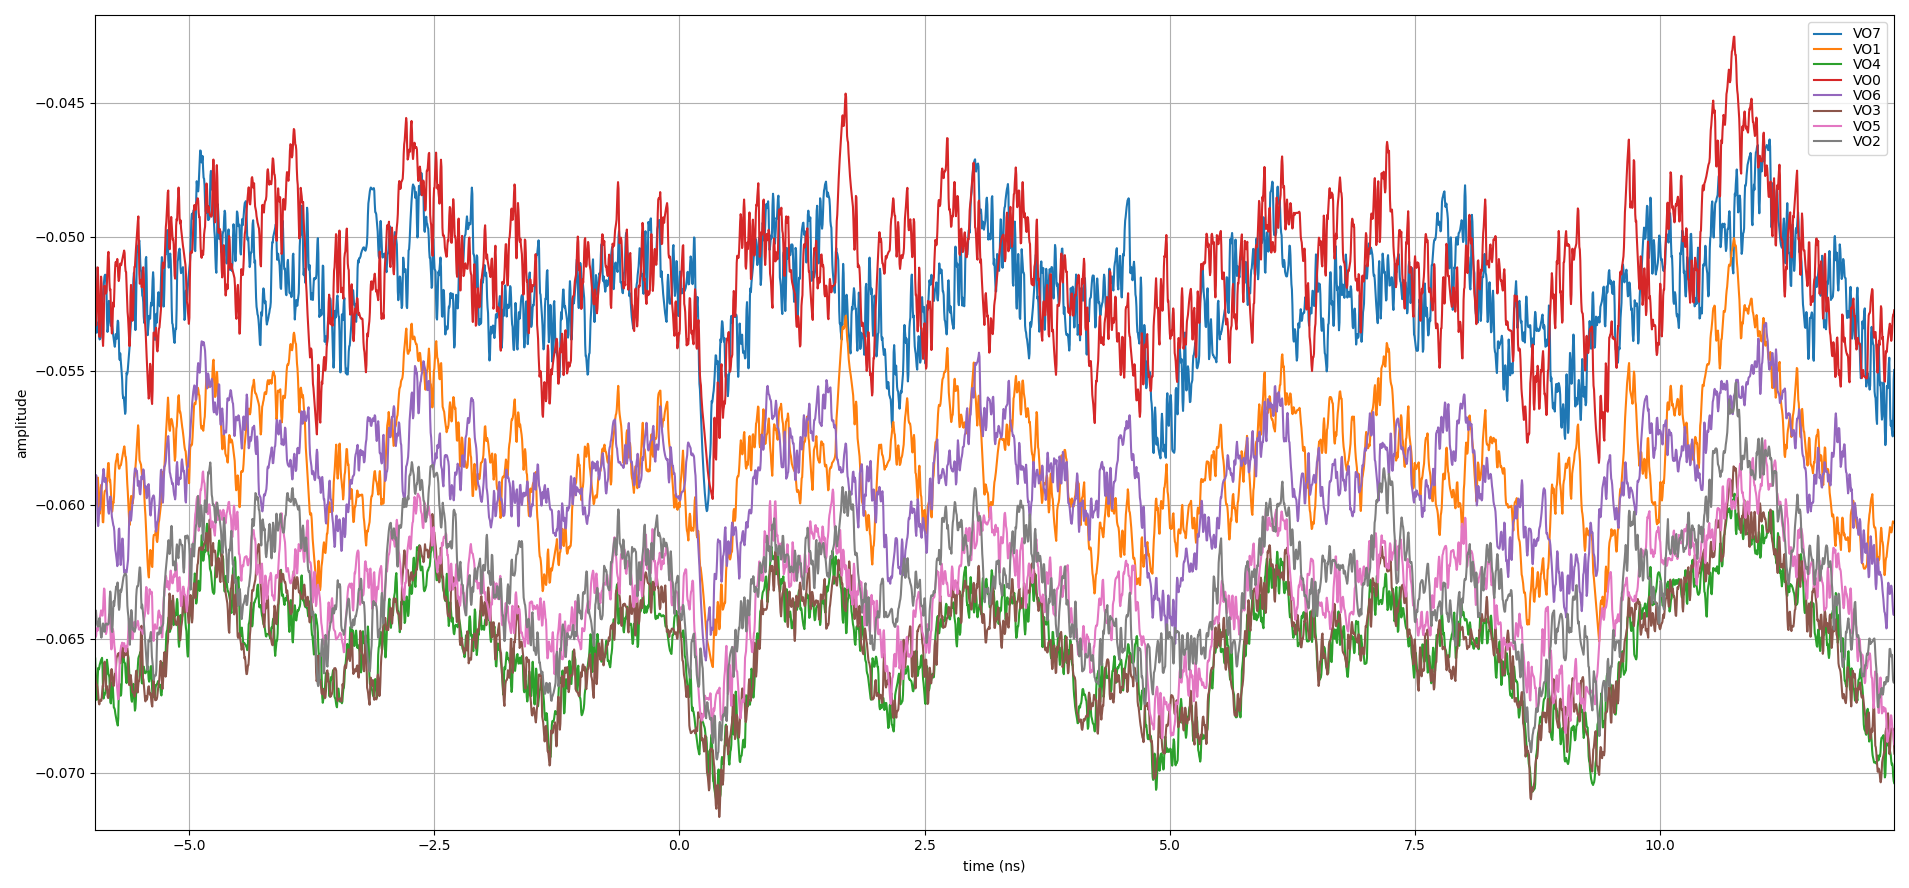
\includegraphics[width=1\columnwidth]{HeftyWBTimeDomainZoomed}

{\footnotesize{}Transient Supply Noise}{\footnotesize\par}
\end{figure}


\column{0.4\textwidth}

\begin{figure}
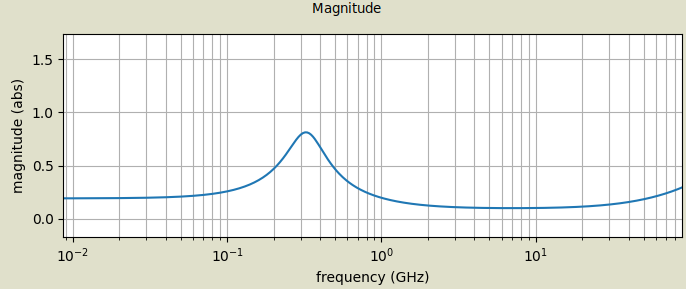
\includegraphics[width=1\columnwidth]{PDNImpedance}

{\footnotesize{}PDN Impedance}{\footnotesize\par}
\end{figure}

\begin{center}
\begin{figure}
\begin{centering}
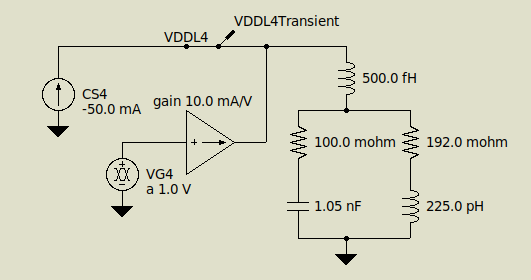
\includegraphics[width=1\columnwidth]{PDNApproximation}
\par\end{centering}
{\footnotesize{}PDN Approximate Circuit (with Transients)}{\footnotesize\par}
\end{figure}
\par\end{center}

\end{columns}

\end{frame}
%
\begin{frame}{Missing from the PDN Simulation}

What went well:
\begin{itemize}
\item HFSS does a great job of producing the simulation (the Z-parameters)
of the PDN from geometry and material properties.
\item The SignalIntegrity software allowed for fitting and transient simulation
(waveform generation).
\end{itemize}
What is missing?
\begin{block}{The Analysis!}

The user is left with some waveforms that are begging for parameters
and measurements.
\end{block}
\end{frame}
%
\begin{frame}{Transfer Matrices Processing}
\begin{columns}

\column{0.5\textwidth}

test

\column{0.5\textwidth}

{\scriptsize{}$\left(\begin{array}{cccc}
H_{11} & H_{12} & \cdots & H_{1K}\\
H_{21} & H_{22} & \cdots & H_{2K}\\
\vdots & \vdots & \ddots & \vdots\\
H_{M1} & H_{M2} & \cdots & H_{MK}
\end{array}\right)\cdot\left(\begin{array}{c}
VS_{1}\\
VS_{2}\\
\vdots\\
VS_{K}
\end{array}\right)=\text{\ensuremath{\left(\begin{array}{c}
VO_{1}\\
VO_{2}\\
\vdots\\
VO_{M}
\end{array}\right)}}$}{\scriptsize\par}
\end{columns}

\end{frame}
%
\begin{frame}[allowframebreaks=1.0]{The Case for Simulation and Oscilloscopes}
\begin{itemize}
\item In today's world, the design phase always begins with simulation.
And, when IC designs are involved, there is a long time between the
conceptual design (that is simulated) and the actual instance of hardware
(that is measured).
\item Also, when trying to understand the implications of various design
choices at a system level, simulations are performed with each of
the constituent elements to determine interoperability and final system
performance.
\item It is common, therefore, to simulate constantly (similar to the ``performance
roll-up'' that we have employed in the TechDev group)
\end{itemize}
\begin{exampleblock}{Diagram}

Picture of the design flow showing iteration and simulation
\end{exampleblock}
\end{frame}
%
\begin{frame}[allowframebreaks=1.0]{Slide}
\begin{itemize}
\item template
\end{itemize}
\end{frame}
%
\begin{frame}[allowframebreaks=1.0]{Slide}
\begin{itemize}
\item template
\end{itemize}
\end{frame}
%
\begin{frame}[allowframebreaks=1.0]{Slide}
\begin{itemize}
\item template
\end{itemize}
\end{frame}
%
\begin{frame}[allowframebreaks=1.0]{Slide}
\begin{itemize}
\item template
\end{itemize}
\end{frame}
%
\begin{frame}[allowframebreaks=1.0]{Slide}
\begin{itemize}
\item template
\end{itemize}
\end{frame}
%
\begin{frame}[allowframebreaks=1.0]{Slide}
\begin{itemize}
\item template
\end{itemize}
\end{frame}
%
\begin{frame}[allowframebreaks=1.0]{Slide}
\begin{itemize}
\item template
\end{itemize}
\end{frame}
%
\begin{frame}[allowframebreaks=1.0]{Slide}
\begin{itemize}
\item template
\end{itemize}
\end{frame}
%
\begin{frame}[allowframebreaks=1.0]{Slide}
\begin{itemize}
\item template
\end{itemize}
\end{frame}
%
\begin{frame}[allowframebreaks=1.0]{Slide}
\begin{itemize}
\item template
\end{itemize}
\end{frame}
%
\begin{frame}[allowframebreaks=1.0]{Slide}
\begin{itemize}
\item template
\end{itemize}
\end{frame}
%
\begin{frame}[allowframebreaks=1.0]{Slide}
\begin{itemize}
\item template
\end{itemize}
\end{frame}
%
\begin{frame}[allowframebreaks=1.0]{Slide}
\begin{itemize}
\item template
\end{itemize}
\end{frame}
%
\begin{frame}[allowframebreaks=1.0]{Slide}
\begin{itemize}
\item template
\end{itemize}
\end{frame}
%
\begin{frame}[allowframebreaks=1.0]{Slide}
\begin{itemize}
\item template
\end{itemize}
\end{frame}
%
\begin{frame}[allowframebreaks=1.0]{Slide}
\begin{itemize}
\item template
\end{itemize}
\end{frame}
%
\begin{frame}[allowframebreaks=1.0]{Slide}
\begin{itemize}
\item template
\end{itemize}
\end{frame}
%
\begin{frame}[allowframebreaks=1.0]{Slide}
\begin{itemize}
\item template
\end{itemize}
\end{frame}
%
\begin{frame}[allowframebreaks=1.0]{Slide}
\begin{itemize}
\item template
\end{itemize}
\end{frame}
%
\begin{frame}[allowframebreaks=1.0]{Slide}
\begin{itemize}
\item template
\end{itemize}
\end{frame}
%
\begin{frame}[allowframebreaks=1.0]{Slide}
\begin{itemize}
\item template
\end{itemize}
\end{frame}
%
\begin{frame}[allowframebreaks=1.0]{Slide}
\begin{itemize}
\item template
\end{itemize}
\end{frame}
%
\begin{frame}[allowframebreaks=1.0]{Slide}
\begin{itemize}
\item template
\end{itemize}
\end{frame}
%
\begin{frame}[allowframebreaks=1.0]{Slide}
\begin{itemize}
\item template
\end{itemize}
\end{frame}
%
\begin{frame}[allowframebreaks=1.0]{Slide}
\begin{itemize}
\item template
\end{itemize}
\end{frame}
%
\begin{frame}[allowframebreaks=1.0]{SignalIntegrity Elements Demonstrated}
\begin{itemize}
\item The viewing and resampling of s-parameters for signal integrity.
\item The impedance profile.
\item Impedance peeling de-embedding techniques.
\item Standard de-embedding techniques (for the peeled launch and the fixture).
\item S-parameter system solutions.
\item RLGC transmission line model fitting.
\item Physicality enforcements.
\end{itemize}
\begin{block}{}
In the process of performing this example, we will learn some things
about s-paramters in signal integrity applications.
\end{block}
\end{frame}
%

\section{Measurement Problem}
\begin{frame}{Measurement Problem}
\begin{itemize}
\item In HDMI (and many cable measurements), the cable has some sort of
specialized connector.
\item Most test instruments expose some sort of coaxial connector, like
SMA, $3.5\thinspace\mathrm{mm}$, or K ($2.92\thinspace\mathrm{mm})$.
\item To facilitate a connection, a text fixture is used with the test instrument
connectors on one side and the cable connector on the other.
\item Sometimes, if the fixture is of extremely high quality, its effects
are ignored.
\item Most often, the fixture is de-embedded, or removed from the measurement,
exposing only a measurement of the cable.
\item There are many options for de-embedding.
\end{itemize}
\end{frame}
%
\begin{frame}{Pictures}

Below are pictures of two measurements that will be made. One of the
measurements is made one time, the other is made for each cable.
\begin{columns}

\column{0.5\textwidth}

\noindent\fbox{\begin{minipage}[c][1in]{1\columnwidth - 2\fboxsep - 2\fboxrule}%
picture of the 1x thru%
\end{minipage}}

The $1\times$ thru is measured once, and is used for de-embedding.

\column{0.5\textwidth}

\noindent\fbox{\begin{minipage}[c][1in]{1\columnwidth - 2\fboxsep - 2\fboxrule}%
picture of the fixture and cable.%
\end{minipage}}

Measurements are made of the fixtures plus the cable.
\end{columns}

\end{frame}
%
\begin{frame}[allowframebreaks=0.75]{$1\times$ Thru Examination}

\framesubtitle{open HDMIFixtureThru.s2p}
\begin{itemize}
\item The $1\times$ thru has launches on each side and a trace in the middle.
\item The actual trace will have a launch on one side and presumably the
same middle trace.
\item Examination of the trace measurements taken to $40\thinspace\mathrm{GHz}$
instantly reveal that $20\thinspace\mathrm{GHz}$ is more reasonable.
\item The launch is slightly inductive (at the coax to microstrip transition)
followed by slight excess capacitance.
\item The trace is $442\thinspace\mathrm{ps}$ long and is approximately
$52\thinspace\Omega$.
\item The frequency resolution is adequate (maybe too fine).
\item The $S_{11}$ magnitude is about $-20\thinspace\mathrm{dB}$ to $20\thinspace\mathrm{GHz}$
\textendash{} not great, but not terrible.
\item The s-parameters are slightly non-passive and can be corrected.
\end{itemize}
\end{frame}
%
\begin{frame}{Raw Cable Measurement Examination}
\begin{itemize}
\item The port numbering can be determined.
\begin{itemize}
\item $S_{41}$ confirms 1\textendash 4 connection (as does $S_{32}$).
\item $S_{31}$ confirms coupling (note the phase) as does $S_{21}$.
\item $S_{42}$ compared to $S_{43}$ confirm that 3 and 4 on same side
(as well as 1 and 2).
\end{itemize}
\item The s-parameters are slightly non-passive and can be corrected.
\end{itemize}
\end{frame}
%
\begin{frame}{Raw Cable and Trace Comparison}
\end{frame}
%

\section{Summary}
\begin{frame}{Summary}
\end{frame}
%

\end{document}
